%\documentclass[cjk,slidestop,compress,brown]{beamer}
\documentclass[cjk,t,compress]{beamer}
%\documentclass[cjk,slidestop,compress]{beamer}

\usepackage{amsmath}
\usepackage{amssymb}
\usepackage{amsthm}

\mode<presentation>
{
%	\usetheme{Hannover}
%	\usetheme{Goettingen}
%   \usetheme{Boadilla}
%	\usetheme{Szeged}
%	\usetheme{Singapore}
%	\usetheme{CambridgeUS}
	\setbeamercovered{dynamic}
	\usefonttheme[hoptionsi]{serif}
%  \usecolortheme[green]{structure}
}

\usepackage{amsmath}
\usepackage{amssymb}
\usepackage{amsthm}
\usepackage{mathtools}

\mode<presentation>
{
%	\usetheme{Hannover}
%	\usetheme{Goettingen}
%   \usetheme{Boadilla}
%	\usetheme{Szeged}
%	\usetheme{Singapore}
%	\usetheme{CambridgeUS}
	\setbeamercovered{dynamic}
	\usefonttheme[hoptionsi]{serif}
%  \usecolortheme[green]{structure}
}

\usepackage[latin1]{inputenc}
\usepackage[spanish]{babel}
%\usepackage{xcolor}
%\usepackage[dvips]{color}
%\usepackage{multicol}
%\usepackage{subfigure}

\definecolor{MyDarkBlue}{rgb}{0 0.08 0.45}
\definecolor{MyDarkOrange}{rgb}{1 0.5 0}
\definecolor{MyDarkGreen}{rgb}{0 0.25 0}
\definecolor{MyDarkTerracota}{rgb}{0.5 0 0}
\definecolor{MyDarkGrey}{rgb}{0.25 0.25 0.25}

% ---------------------------------------------
%				Fields
% ---------------------------------------------
\newcommand{\Indicator}{\operatorname{\mathds{1}}}
\newcommand{\Indic}{\operatorname{\field{I}}}
\newcommand{\field}[1]{\mathbb{#1}} 
\newcommand{\C}{\field{C}}
\newcommand{\E}{\field{E}} 
\newcommand{\R}{\field{R}}
\newcommand{\inccoin}{\Delta c}
\newcommand{\incy}{\Delta y}

% ---------------------------------------------
%				Observables
% ---------------------------------------------
\newcommand{\barx}{\bar{x}}
\newcommand{\barX}{\bar{X}}
\newcommand{\boldc}{\boldsymbol{c}}
\newcommand{\boldC}{\boldsymbol{C}}
\newcommand{\boldm}{\boldsymbol{m}}
\newcommand{\boldM}{\boldsymbol{M}}
\newcommand{\boldr}{\boldsymbol{r}}
\newcommand{\boldR}{\boldsymbol{R}}
\newcommand{\boldx}{\boldsymbol{x}}
\newcommand{\boldX}{\boldsymbol{X}}
\newcommand{\boldy}{\boldsymbol{y}} 
\newcommand{\boldS}{\boldsymbol{S}}
\newcommand{\boldu}{\boldsymbol{u}} 
\newcommand{\boldU}{\boldsymbol{U}}
\newcommand{\boldzero}{\boldsymbol{0}} 
\newcommand{\boldA}{\boldsymbol{A}} 
\newcommand{\boldW}{\boldsymbol{W}}

% ---------------------------------------------
%				Parameters
% ---------------------------------------------
\newcommand{\piexp}{\pi^{e}} 
\newcommand{\pidelta}{\delta^{\pi}} 

\newcommand{\rhoexp}{\rho^{e}} 
\newcommand{\rhodelta}{\delta^{\rho}} 

\newcommand{\tauexp}{\tau^{e}} 
\newcommand{\taudelta}{\delta^{\tau}} 

\newcommand{\thetaexp}{\theta^{e}} 
\newcommand{\thetadelta}{\delta^{\theta}} 

\newcommand{\tk}{t:(t+k)} 

\newcommand{\boldlambda}{\boldsymbol{\lambda}} 
\newcommand{\boldLambda}{\boldsymbol{\Lambda}} 
\newcommand{\boldmu}{\boldsymbol{\mu}} 
\newcommand{\boldMu}{\boldsymbol{\Mu}} 
\newcommand{\boldsigma}{\boldsymbol{\sigma}} 
\newcommand{\boldSigma}{\boldsymbol{\Sigma}} 
\newcommand{\boldphi}{\boldsymbol{\phi}} 
\newcommand{\boldPhi}{\boldsymbol{\Phi}} 
\newcommand{\boldbeta}{\boldsymbol{\beta}}
\newcommand{\boldBeta}{\boldsymbol{\Beta}}
\newcommand{\boldtheta}{\boldsymbol{\theta}}
\newcommand{\boldTheta}{\boldsymbol{\Theta}}
\newcommand{\bolds}{\boldsymbol{s}} 
%\newcommand{\boldS}{\boldsymbol{S}} 

%   --------------------------------
%               Notation
%   --------------------------------
\newcommand{\lik}{\mathrm{lik}}
\newcommand{\diagop}{\text{diag}} 
\newcommand{\logistic}{\operatorname{\text{logistic}}}
\newcommand{\logit}{\operatorname{\text{logit}}}
\newcommand{\dom}{\operatorname{\text{dom}}}
\newcommand{\ran}{\operatorname{\text{ran}}}
\renewcommand{\inf}{\operatorname{\text{inf}}}
\newcommand{\ind}{\operatorname{\text{ind}}}
\newcommand{\iid}{\operatorname{\text{iid}}}
\newcommand{\cind}{\operatorname{\text{c.i.}}}
\newcommand{\wport}{\text{w}}

\renewcommand{\Pr}{\field{P}}
\newcommand{\dd}{\mathrm{d}}
\newcommand{\Borel}{\operatorname{\mathscr{B}}}
\newcommand{\Filtration}{\operatorname{\mathscr{F}}}
\newcommand{\expec}{\operatorname{\field{E}}}
%\newcommand{\media}{\operatorname{\text{media}}}
%\newcommand{\moda}{\operatorname{\text{moda}}}
%\renewcommand{\var}{\operatorname{\text{var}}}
%\newcommand{\prec}{\operatorname{\text{prec}}}
%\newcommand{\cov}{\operatorname{\text{cov}}}
%\newcommand{\corr}{\operatorname{\text{corr}}}
%\newcommand{\varmodel}{\operatorname{\text{VAR}}}

\renewcommand{\sin}{\operatorname{\text{sin}}}
\renewcommand{\cos}{\operatorname{\text{cos}}}
\renewcommand{\tan}{\operatorname{\text{tan}}}
\renewcommand{\arctan}{\operatorname{\text{arctan}}}
\renewcommand{\exp}{\operatorname{\text{exp}}}
\renewcommand{\log}{\operatorname{\text{log}}}
\renewcommand{\arg}{\operatorname{\text{arg}}}
\renewcommand{\min}{\operatorname{\text{min}}}
\renewcommand{\max}{\operatorname{\text{max}}}
\renewcommand{\lim}{\operatorname{\text{lim}}}
\newcommand{\limite}{\operatornamewithlimits{lim}}
\renewcommand{\det}{\operatorname{\text{det}}}
\renewcommand{\dim}{\operatorname{\text{dim}}}
\newcommand{\sign}{\operatorname{\text{sign}}}
\newcommand{\argmax}{\operatornamewithlimits{arg\,max}}
\newcommand{\argmin}{\operatornamewithlimits{arg\,min}}
\newcommand{\diagbloq}{\operatorname{\text{diagbloq}}}
\newcommand{\rr}{\operatorname{\textsc{R}}}

\newcommand{\ie}{{\it i.e. }} 
\newcommand{\aka}{{\it a.k.a. }} 
\newcommand{\eg}{{\it e.g. }} 
\newcommand{\ala}{{\it \`{a}~la }} 
\newcommand{\visavis}{{\it vis-\`{a}-vis }}

\newcommand{\inpc}{\text{INPC}}
\newcommand{\igae}{\text{IGAE}}
\newcommand{\pib}{\text{PIB}}
\newcommand{\tiie}{\text{TIIE}}
\newcommand{\export}{\text{Exportaciones}}
\newcommand{\import}{\text{Importaciones}}
\newcommand{\usip}{\text{IP}^{\usa}}
\newcommand{\remMS}{\text{Rem}^{\usa}}
\newcommand{\itaen}{\text{ITAE}}
\newcommand{\itaee}{\text{ITAEE}}
\newcommand{\usa}{\text{EEUU}}
\newcommand{\dsge}{\operatornamewithlimits{DSGE}}

% ---------------------------------------------
%				Distributions
% ---------------------------------------------

\newcommand{\WiD}{\operatorname{\text{Wi}}}
\newcommand{\WiInvD}{\operatorname{\text{Wi-Inv}}}
\newcommand{\WeD}{\operatorname{\text{We}}}
\newcommand{\WeNormD}{\operatorname{\text{We-N}}}
\newcommand{\ExpD}{\operatorname{\text{Exp}}}
\newcommand{\GeoD}{\operatorname{\text{Geo}}}
\newcommand{\StD}{\operatorname{\text{St}}}
\newcommand{\NormD}{\operatorname{\text{N}}}
\newcommand{\GaD}{\operatorname{\text{Ga}}}
\newcommand{\BerD}{\operatorname{\text{Ber}}}
\newcommand{\BinD}{\operatorname{\text{Bin}}}
\newcommand{\BeD}{\operatorname{\text{Be}}}
\newcommand{\UniD}{\operatorname{\text{U}}}
\newcommand{\DirD}{\operatorname{\text{Dir}}}
\newcommand{\IG}{\operatorname{\text{InG}}}
\newcommand{\IncGa}{\operatorname{\text{IGa}}}
\newcommand{\IGa}{\operatorname{\text{InGa}}}
\newcommand{\PoD}{\operatorname{\text{Po}}}
\newcommand{\BS}{\operatorname{\text{BS}}}
\newcommand{\DP}{\operatorname{\text{DP}}}


%   --------------------------------
%               Directories
%   --------------------------------
\graphicspath{{../figures/}}
\DeclareGraphicsExtensions{.pdf,.jpeg,.png,.jpg}

\title[C\'alculo Actuarial III]
{	ACT-11302: C\'alculo Actuarial III\\
	{\large Sesion 09b: Primas de riesgo}
}

\author[Mart\'inez-Ovando]{
{	\footnotesize
	\textcolor{MyDarkGreen}{Juan~Carlos Mart\'inez-Ovando}}
}

\institute[ITAM]
{	\textcolor{MyDarkGrey}{
	ITAM}
}

\date[ ] % (optional)
{	\scriptsize
	\textcolor{MyDarkGrey}{Oto\~no 2019}
}

%	--------------------------------------------
%									Titlepage
%	--------------------------------------------
\begin{document}
\sffamily
%	-------------		FRAME		--------------------
\begin{frame}[fragile]
	\frametitle{}
	\titlepage
\end{frame}

%
%	Section: Monto agregado de siniestros
%
\section{1. Prima de riesgo}
%	-------------		FRAME		--------------------
\begin{frame}[fragile]
	\frametitle{}
	\vspace{5.5cm}
	\begin{flushright}
		\textcolor{MyDarkBlue}{\Large \bf 1. Prima de riesgo}
	\end{flushright}
\end{frame}

%
%	Sub-section: Antecedentes
%
\subsection{1.1 Prima de riesgo: Antecedentes}
%	-------------		FRAME		--------------------
\begin{frame}[fragile]
	\frametitle{1.1 Prima de riesgo: Antecedentes}
	\scriptsize  	
		
		\vspace{0.4cm}
		\begin{block}<+->{Definici\'on}
		\vspace{0.3cm}
		\begin{itemize}
		 \item La \textcolor{blue}{\bf prima de riesgo} es el monto que un asegurado paga por la cobertura parcial o total contra un riesgo.
		
		 \item Denotamos por $\Pi_S$ a la prima que una aseguradora cobra para cubrir el riesgo $S$.
		 \item El riesgo $S$ es una variable aleatoria,
		 
		 \item[] as\'i, $\Pi_S$ es una funci\'on de la v.a. $S$, i.e.
		\begin{equation}
			\Pi_S=\phi(S),
			\nonumber
		\end{equation}
		para alguna funci\'on $\phi$, la cual define el \textcolor{blue}{\bf principio de c\'alculo de primas}.
		\end{itemize}
		\end{block}  		
				
\end{frame}

%	-------------		FRAME		--------------------
\begin{frame}[fragile]
	\frametitle{1.1 Prima de riesgo: Antecedentes}
	\scriptsize  	
		
		\begin{block}<+->{}
		\vspace{0.1cm}
		\begin{figure}[hbtp]
		\caption{Principio de c\'alculo de primas}
		\centering
		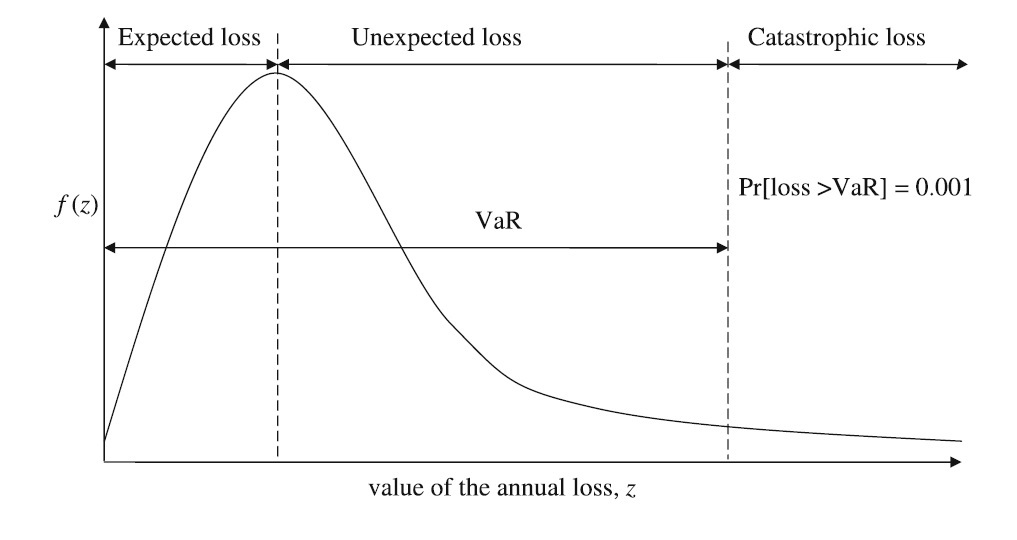
\includegraphics[scale=0.41]{Figuras/Loss_distribution.jpeg}
		\end{figure}
		{\tiny Fuente: Deelstra et al.}
		\end{block}  		
	
\end{frame}

%
%	Sub-section: Propiedades
%
\subsection{1.2 Prima de riesgo: Propiedades}
%	-------------		FRAME		--------------------
\begin{frame}[fragile]
	\frametitle{1.2 Prima de riesgo: Propiedades}
	\scriptsize  	
		
		\vspace{0.2cm}
		\begin{block}<+->{a) No negatividad}
		\vspace{0.1cm}
		Es deseable que la prima de riesgo no sea menor que la p\'erdida esperada, i.e.
		\begin{equation}
			\Pi_S \geq \expec(S).
		\end{equation}
		\textcolor{MyDarkGreen}{Esta propiedad es fundamental para la {\it teor\'ia de ruina}.}
		\end{block}  		

		\vspace{0.2cm}
		\begin{block}<+->{b) Aditividad}
		\vspace{0.1cm}
		Para dos riesgos independientes, $S_1$ y $S_2$, se desea,
		\begin{equation}
			\Pi_{S_1+S_2} = \Pi_{S_1}+ \Pi_{S_2}.
		\end{equation}
		\textcolor{MyDarkGreen}{Esta propiedad es fundamental para la combinaci\'on de riesgos.}
		\end{block}  		
	
\end{frame}

%	-------------		FRAME		--------------------
\begin{frame}[fragile]
	\frametitle{1.2 Prima de riesgo: Propiedades}
	\scriptsize  	
		
		\vspace{0.2cm}
		\begin{block}<+->{c) Invarianza en escala}
		\vspace{0.1cm}
		Si $S$ es un riesgo y $\alpha$ es un escalar positivo (fijo y conocido), es deseable,
		\begin{equation}
			\Pi_{\alpha S} \geq \alpha \Pi_{S}.
		\end{equation}
		\textcolor{MyDarkGreen}{Esta propiedad es fundamental para manipular primar de riesgo en unidades monetarias.}
		\end{block}  		

		\vspace{0.2cm}
		\begin{block}<+->{d) Consistencia}
		\vspace{0.1cm}
		Si $S$ es un riesgo y $\delta$ es un escalar positivo (fijo y conocido), se desea,
		\begin{equation}
			\Pi_{S+\delta} = \Pi_{S}+\delta.
		\end{equation}
		\textcolor{MyDarkGreen}{Esta propiedad se refiere a la invarianza ante traslaciones.}
		\end{block}  		
	
\end{frame}

%	-------------		FRAME		--------------------
\begin{frame}[fragile]
	\frametitle{1.2 Prima de riesgo: Propiedades}
	\scriptsize  	
		
		\vspace{0.2cm}
		\begin{block}<+->{e) No estafa}
		\vspace{0.1cm}
		En caso de existir un monto m\'aximo de reclamo, $x^{*}$, se desea,
		\begin{equation}
			\Pi_{S} \leq x^{*}.
		\end{equation}
		En este caso, $\Pi_{S}$ se refiere a la prima se riesgo individual.		
		
		\textcolor{MyDarkGreen}{Esta propiedad es fundamental para efectuar el seguro.}
		\end{block}  		

\end{frame}

%
%	Sub-section: Ejemplos
%
\subsection{1.3 Prima de riesgo: Ejemplos}
%	-------------		FRAME		--------------------
\begin{frame}[fragile]
	\frametitle{1.3 Prima de riesgo: Ejemplos}
	\scriptsize  	
		
		\vspace{0.2cm}
		\begin{block}<+->{I. Prima de riesgo pura}
		\vspace{0.1cm}
		Es la prima de riesgo b\'asica, se define como la p\'erdida esperada, i.e.
		\begin{equation}
			\Pi_S = \expec(S).
		\end{equation}
		
		\begin{itemize}
		  \item No es atractiva para la aseguradora.
		  \item No tiene margen de ganacia (o negocio).
		  \item Alta exposici\'on a riesgo de ruina.
		  \item A pesar de lo anterior, satisface los 5 principios anteiores. 
		\end{itemize}
		\end{block}  		

\end{frame}

%	-------------		FRAME		--------------------
\begin{frame}[fragile]
	\frametitle{1.3 Prima de riesgo: Ejemplos}
	\scriptsize  	
		
		\vspace{0.2cm}
		\begin{block}<+->{II. Prima de riesgo basada en el principio del valor esperado}
		\vspace{0.1cm}
		Es la prima de riesgo b\'asica, se define como la p\'erdida esperada ajustada por un margen de aceptaci\'on de riesgo, $\theta>0$, i.e.
		\begin{equation}
			\Pi_S = (1+\theta)\expec(S).
		\end{equation}
		\textcolor{blue}{El factor $\theta$ se conoce como factor de carga o ajuste. Representa el nivel de aversión al riesgo de la aseguradora.}
		
		\begin{itemize}
		  \item Satisface los principios deseables salvo el de consistencia, pues
		  $$\Pi_{S+\delta} > \Pi_{S}+\delta,$$
		  y el de {\bf no estafa}.
		  \item Es m\'as conservadora que la prima de riesgo b\'asica.
		  \item Asigna la misma prima a todos los riesgos con la "misma" p\'erdida esperada. 
		  \item No toma en cuenta momentos mayores al primero.
		\end{itemize}
		\end{block}  		

\end{frame}

%	-------------		FRAME		--------------------
\begin{frame}[fragile]
	\frametitle{1.3 Prima de riesgo: Ejemplos}
	\scriptsize  	
		
		\vspace{0.2cm}
		\begin{block}<+->{III. Prima de riesgo basada en el principio de la varianza}
		\vspace{0.1cm}
		Es la prima de riesgo b\'asica, se define como la p\'erdida esperada ajustada por un margen de aceptaci\'on de riesgo, $\alpha>0$ en funci\'on de su varianza, i.e.
		\begin{equation}
			\Pi_S = \expec(S)+\alpha var(S).
		\end{equation}
		\textcolor{blue}{En este caso, el factor de recarga es un m\'ultiplo del segundo momento del riesgo.}
		
		\begin{itemize}
		  \item Satisface los principios deseables salvo el de invarianza en escala, pues
		  $$\Pi_{\gamma S} \neq \gamma \Pi_{S},$$
		  para $\gamma>0$, y el de {\bf no estafa}.
		  \item Es m\'as conservadora que la prima de riesgo b\'asica.
		  \item Asigna primas diferenciadas en funci\'on del segundo momento del riesgo. 
		  \item No toma en cuenta momentos mayores al segundo momento.
		\end{itemize}
		\end{block}  		

\end{frame}

%	-------------		FRAME		--------------------
\begin{frame}[fragile]
	\frametitle{1.3 Prima de riesgo: Ejemplos}
	\scriptsize  	
		
		\vspace{0.2cm}
		\begin{block}<+->{IV. Prima de riesgo basada en el principio de utilidad cero}
		\vspace{0.1cm}
		La aseguradora tiene una preferencia de riesgos dada por la funci\'on de utilidad $u(\cdot)$ (con $u'(\cdot)>0$ y $u''(\cdot)<0$). Es deseable as\'i que $\Pi_{S}$ sea tal que, 
		\begin{equation}
			u(W) = \expec\left(u\left(W+\Pi_{S}-X\right)\right),
		\end{equation}
		donde $W$ es el excedente de la aseguradora.
		\newline
		\textcolor{blue}{En este caso, el factor de recarga es un m\'ultiplo del segundo momento del riesgo.}
		
		\begin{itemize}
		  \item Es atractiva, pues incorpora informaci\'on acerca de todos los momentos del riesgo $S$.
		  \item Est\'a en funci\'on del margen de excedente de la aaseguradora.
		  \item Satisface los principios desables, salvo el de invarianza en escala, pues
		  $$\Pi_{\gamma S}\neq \gamma \Pi_{S}.$$
		\end{itemize}
		\end{block}  		

\end{frame}

%	-------------		FRAME		--------------------
\begin{frame}[fragile]
	\frametitle{1.3 Prima de riesgo: Ejemplos}
	\scriptsize  	
		
		\vspace{0.2cm}
		\begin{block}<+->{V. Prima de riesgo basada en el principio de prima ajustada}
		\vspace{0.1cm}
		Suponiendo que el riesgo $S$ se describe con $F_{S}(S)$, se define
		\begin{equation}
			\Pi_{S} = \int_{0}^{\infty}\left(1-F_{S}(S)\right)^{1/\rho}\dd x,
		\end{equation}
		donde $\rho\geq 1$ es el \'indice de riesgo.
		\newline
		\textcolor{blue}{En este caso, se da un mayor peso a los riesgos extremos en $S$ (cola derecha de la distribuci\'on $F_{S}$).}
		
		\begin{itemize}
		  \item Es la prima de riesgo base inducida por la transformaci\'on $$1-H_{S}(S)=(1-F_{S}(S))^{1/\rho}.$$
		  \item Si $F_S$ es absolutamente continua, entonces $$h_{S}(S)=\frac{1}{\rho}\left(1-F_{S}(S)\right)^{1/\rho-1}f_{S}(S),$$
		  i.e. la densidad de la modificaci\'on es funci\'on ponderada de $f_{S}$.
		  \item Satisface los 5 principios desables, salvo el de aditividad.
		\end{itemize}
		\end{block}  		

\end{frame}

%	-------------		FRAME		--------------------
\begin{frame}[fragile]
	\frametitle{1.3 Prima de riesgo: Ejemplos}
	\scriptsize  	
	
	\vspace{0.2cm}
	\begin{block}<+->{VI. Prima de riesgo basada en el principio exponencial}
		\vspace{0.1cm}
		Suponiendo que el riesgo $S$ se describe con $F_{S}(S)$, se define
		\begin{equation}
		\Pi_{S} = \frac{1}{\alpha}\log\left(\expec _{F_{S}}(e^{\alpha S})\right),
		\end{equation}
		donde $\alpha > 0$ es el par\'ametro de aversi\'on al riesgo.
		\newline
		\textcolor{blue}{Esta prima asigna una mayor probabilidad a los riesgos extremos en $S$ (cola derecha de la distribuci\'on $F_{S}$).}
		
		\begin{itemize}
			\item La prima se riesgo ser\'a grande cuando $\alpha$ lo sea. Cuando $\alpha$ sea cercana a cero se aproximar\'a a la prima se riesgo pura.
			\item El principio exponencial coincide con el de utilidad cero empleando una funci\'on de utilidad exponencial ($\alpha$ mide el \'indice de aversi\'on al riesgo).
			\item Satisface los 5 principios desables, salvo el de aditividad.
		\end{itemize}
	\end{block}  		
	
\end{frame}

%	-------------		FRAME		--------------------
\begin{frame}[fragile]
	\frametitle{1.3 Prima de riesgo: Ejemplos}
	\scriptsize  	
	
	\vspace{0.2cm}
	\begin{block}<+->{VII. Prima de riesgo basada en el principio de Esscher}
		\vspace{0.1cm}
		Suponiendo que el riesgo $S$ se describe con $F_{S}(S)$, se define
		\begin{equation}
		\Pi_{S} = \frac{\expec _{F_{S}}(Xe^{\alpha S})}{\expec _{F_{S}}(e^{\alpha S})},
		\end{equation}
		donde $\alpha\geq 0$ es el par\'ametro de aversi\'on al riesgo.
		\newline
		\textcolor{blue}{Al igual que la prima anterior, \'esta da un mayor peso a los riesgos extremos en $S$ (cola derecha de la distribuci\'on $F_{S}$).}
		
		\begin{itemize}
			\item Esta distribuci\'on se puede definir alternativamente como el valor esperado del riesgo $S$ bajo la distribuci\'on modificada
			$$G_{S}(S)=\frac{e^{\alpha x}F_{S}(S)}{\int e^{\alpha S}F_{S}(\dd x)}.$$
			\item Satisface los 5 principios desables, salvo el de aditividad.
		\end{itemize}
	\end{block}  		
	
\end{frame}

%
%	Section: Monto agregado de siniestros
%
\section{2. Usos de primas de riesgo}
%	-------------		FRAME		--------------------
\begin{frame}[fragile]
	\frametitle{}
	\vspace{5.5cm}
	\begin{flushright}
		\textcolor{MyDarkBlue}{\Large \bf 2. Usos de primas de riesgo}
	\end{flushright}
\end{frame}

%
%	Sub-section: Antecedentes
%
\subsection{2.1 Usos de primas de riesgo: Coaseguro \'optimo}
%	-------------		FRAME		--------------------
\begin{frame}[fragile]
	\frametitle{2.1 Usos de primas de riesgo: Coaseguro \'optimo}
	\scriptsize  	
		
		\vspace{0.1cm}
		\begin{block}<+->{Planteamiento}
		\vspace{0.3cm}
		\begin{itemize}
		 \item 
		 Coseguro es un acuerdo por el cual varios aseguradores comparten un riesgo.
		 
		 \item Cada participante asume una parte del mismo, por una parte de las primas. 
		 
		 \item Considera $K$ aseguradoras, tal que cada una de ellas fija su prima de riesgo bajo el \textcolor{blue}{\bf principio exponencial} con $\alpha_k$, $k=1,\ldots,K$.
		
		 \item \textcolor{MyDarkTerracota}{?`Cu\'al es el coaseguro \'optimo?}
		\end{itemize}
		\end{block}  		
				
		\vspace{0.1cm}
		\begin{block}<+->{Soluci\'on}
		\vspace{0.3cm}
		\begin{itemize}
		  \item Por la desigualdad de H\"older, asumiendo independencia entre las aseguradoras, se tiene que
		\begin{equation}
		\expec\left(e^{\alpha S}\right) \leq \prod_{k=1}^{K}\expec\left(e^{\alpha_k S_k}\right)^{\alpha/\alpha_k},
		\nonumber
		\end{equation}
		con $1/\alpha=\sum_{k=1}^{K}1/\alpha_k$.
		  \item As\'i, el coaseguro \'optimo se define como
		\begin{equation}
		S_{k}^{*}=\frac{\alpha}{\alpha_k}S.
		\nonumber
		\end{equation}
		\end{itemize}
		\end{block}  	
\end{frame}

%
%	Sub-section: Antecedentes
%
\subsection{2.2 Usos de primas de riesgo: Costo de reaseguro}
%	-------------		FRAME		--------------------
\begin{frame}[fragile]
	\frametitle{1.2 Usos de primas de riesgo: Costo de reaseguro}
	\scriptsize  	
		
		\vspace{0.1cm}
		\begin{block}<+->{Planteamiento}
		\begin{itemize}
		 \item 
		Supongamos que una aseguradora fija su prima de riesgo de acuerdo al \textcolor{blue}{\bf principio de varianza}
		 
		 \item Una reaseguradora participa definiendo su prima de riesgo bajo el mismo principio
		 
		 \item Se propone contratar el riesgo agregado con prioridad $M$ (i.e. se paga el reclamo total que excede $M$) 
		
		 \item \textcolor{MyDarkTerracota}{?`Cu\'al es el impacto del costo del reaseguro en el costo del seguro?}
		\end{itemize}
		\end{block}  		
				
		\vspace{0.1cm}
		\begin{block}<+->{Soluci\'on}
		\vspace{0.3cm}
		\begin{itemize}
		  \item Sin reaseguro, la prima de riesgo de la aseguradora ser\'ia
		\begin{equation}
		\Pi_S = \expec\left(X\right)+\alpha \cdot var\left(X\right),
		\nonumber
		\end{equation}
		para alg\'un $\alpha$ positivo.
		  \item $\Pi^{r}_{S}$ denota la prima de riesgo de la reaseguradora; el costo es transferido, con 
		  \begin{eqnarray}
		  a(S)=\min(S,M) & \text{y} & r(S)=max(S-M,0).
		  \nonumber
		  \end{eqnarray}
		  
		\end{itemize}
		\end{block}  	
\end{frame}

%	-------------		FRAME		--------------------
\begin{frame}[fragile]
	\frametitle{2.2 Usos de primas de riesgo: Costo de reaseguro}
	\scriptsize  	
		
		\vspace{0.1cm}
		\begin{block}<+->{Soluci\'on}
		\vspace{0.3cm}
		\begin{itemize}
		  \item Se cumple
		  \begin{equation}
		 	S = a(S)+r(S).
			\nonumber
		  \end{equation}
		  \item As\'i, la prima de riesgo de la reaseguradora es
		  \begin{eqnarray}
		    \Pi^{r}_{S} 
		    		& = & 
		    		\expec\left(a(S)\right) 
		    		+ \expec \left(r(S)\right)
		    		+ \alpha 
		    		\cdot 
		    		\left( var\left(a(S)\right) + var\left(r(S)\right) \right)
		    		\nonumber \\
		    		& = &
		    		\expec(S) 
		    		+ \alpha \cdot var(S)
		    		- \alpha \cdot cov\left(a(S),r(S)\right). 
		    		\nonumber
		  \end{eqnarray}
		  \item Adem\'as, tenemos,
		  \begin{equation}
		    cov\left(a(S),r(S)\right) = \left(M-\expec(a(s))\right)\expec(r(S)) \geq 0.
		    \nonumber
		  \end{equation}
		  \item Como $M \geq \expec\left(\min(S,M)\right)$,
		  se tiene que 
		  \begin{equation}
		  \Pi_{S} \geq \Pi^{r}_{S}.
		  \nonumber
		  \end{equation}
		\end{itemize}
		\end{block}
		  	
\end{frame}

\end{document}
%
%	--	FIN	--